% Diagrama de blocos/fiação do nó ESP32 (beacon ou coletor). Fonte única: usado em
% schematics/esp32-node/esp32-node.pdf e .png e incluído no relatório (docs/relatorio).
% Compilar: pdflatex esp32-node.tex   (PNG: pdftoppm -r 200 -png -singlefile esp32-node.pdf esp32-node)
\documentclass[tikz,border=6pt]{standalone}
\usepackage[T1]{fontenc}
\usepackage[utf8]{inputenc}
\usepackage{times}
\usetikzlibrary{arrows.meta,positioning,fit,backgrounds}
\begin{document}
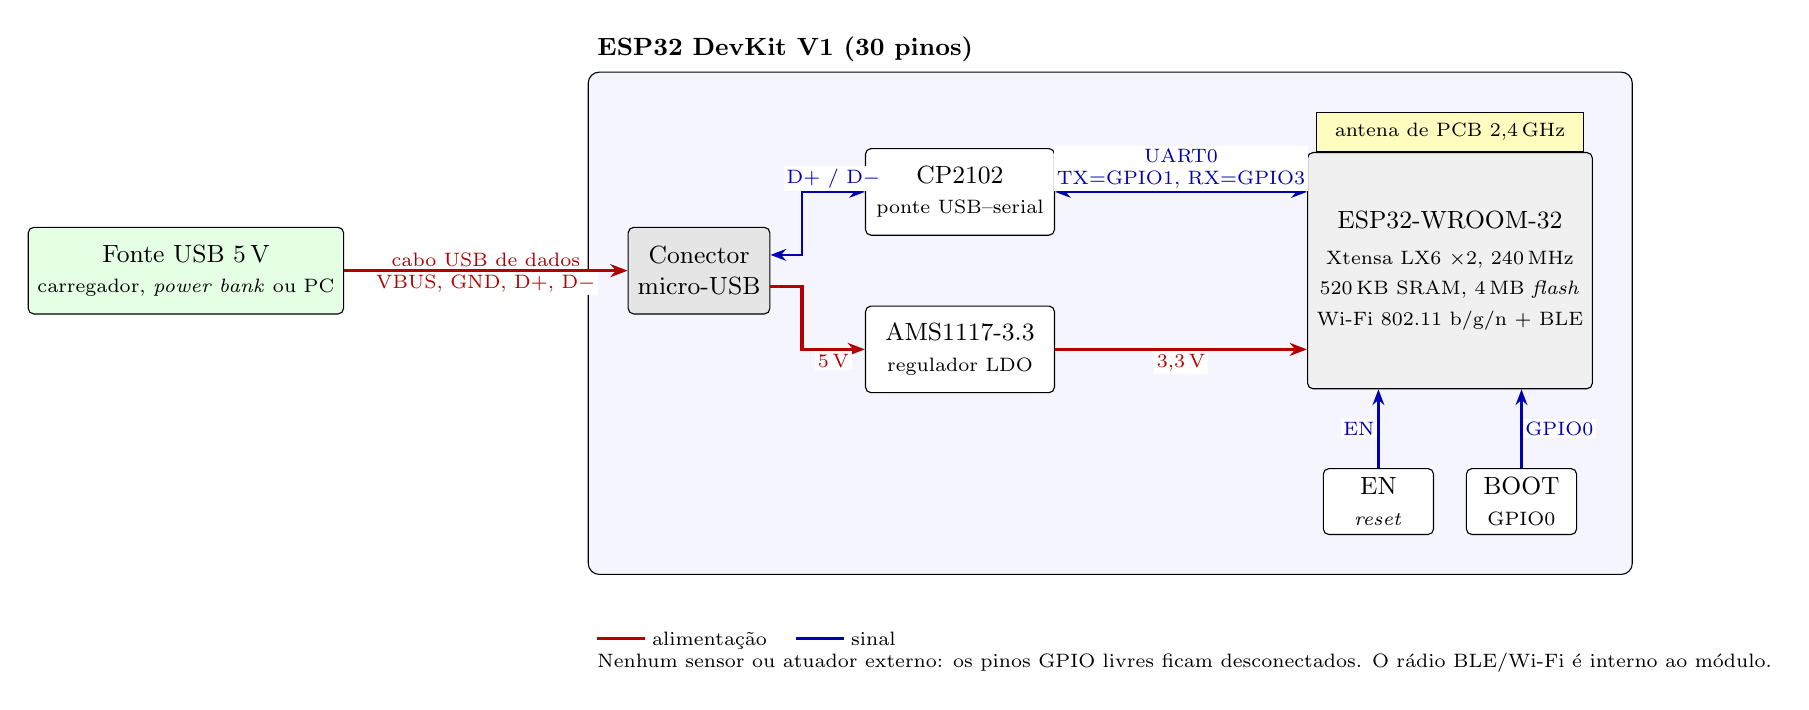
\begin{tikzpicture}[font=\small, node distance=8mm and 12mm,
    blk/.style={draw, rounded corners=2pt, align=center, minimum height=11mm, minimum width=24mm, fill=white},
    pwr/.style={-{Stealth[length=2.2mm]}, very thick, red!70!black},
    gnd/.style={very thick, black},
    sig/.style={{Stealth[length=2mm]}-{Stealth[length=2mm]}, thick, blue!70!black},
    one/.style={-{Stealth[length=2mm]}, thick, blue!70!black},
    lbl/.style={font=\scriptsize, fill=white, inner sep=1pt, align=center}]

  % Fonte externa
  \node[blk, fill=green!10] (src) {Fonte USB 5\,V\\\scriptsize carregador, \textit{power bank} ou PC};

  % Componentes da placa
  \node[blk, right=36mm of src, fill=gray!20, minimum width=18mm] (usb) {Conector\\micro-USB};
  \node[blk, right=of usb, yshift=10mm] (uart) {CP2102\\\scriptsize ponte USB--serial};
  \node[blk, right=of usb, yshift=-10mm] (ldo) {AMS1117-3.3\\\scriptsize regulador LDO};
  \node[blk, right=32mm of uart, yshift=-10mm, minimum height=30mm, minimum width=34mm, fill=gray!12] (mod)
        {ESP32-WROOM-32\\[2pt]\scriptsize Xtensa LX6 $\times$2, 240\,MHz\\\scriptsize 520\,KB SRAM, 4\,MB \textit{flash}\\\scriptsize Wi-Fi 802.11 b/g/n + BLE};
  \node[draw, fill=yellow!25, minimum width=34mm, minimum height=5mm, above=0mm of mod, font=\scriptsize] (ant)
        {antena de PCB 2,4\,GHz};
  \node[blk, below=10mm of mod.south west, anchor=north west, minimum width=14mm, minimum height=7mm, xshift=2mm] (en) {EN\\\scriptsize\textit{reset}};
  \node[blk, below=10mm of mod.south east, anchor=north east, minimum width=14mm, minimum height=7mm, xshift=-2mm] (boot) {BOOT\\\scriptsize GPIO0};

  % Conexões
  \draw[pwr] (src) -- node[lbl, above] {cabo USB de dados} node[lbl, below] {VBUS, GND, D+, D$-$} (usb);
  \draw[pwr] (usb.east) ++(0,-2mm) -- ++(4mm,0) |- node[lbl, pos=0.75, below] {5\,V} (ldo.west);
  \draw[sig] (usb.east) ++(0,2mm) -- ++(4mm,0) |- node[lbl, pos=0.75, above] {D+ / D$-$} (uart.west);
  \draw[pwr] (ldo.east) -- node[lbl, below] {3,3\,V} (ldo.east -| mod.west);
  \draw[sig] (uart.east) -- node[lbl, above] {UART0\\\scriptsize TX=GPIO1, RX=GPIO3} (uart.east -| mod.west);
  \draw[one] (en.north) -- node[lbl, left] {EN} (en.north |- mod.south);
  \draw[one] (boot.north) -- node[lbl, right] {GPIO0} (boot.north |- mod.south);

  % Moldura da placa
  \begin{scope}[on background layer]
    \node[draw, rounded corners=4pt, fill=blue!4, inner sep=5mm, fit=(usb)(uart)(ldo)(mod)(ant)(en)(boot),
          label={[font=\small\bfseries, anchor=south west]north west:ESP32 DevKit V1 (30 pinos)}] (board) {};
  \end{scope}

  % Legenda
  \node[below=6mm of board.south west, anchor=north west, font=\scriptsize, align=left] {%
    \textcolor{red!70!black}{\rule[2pt]{6mm}{1.2pt}} alimentação \quad
    \textcolor{blue!70!black}{\rule[2pt]{6mm}{1pt}} sinal\\
    Nenhum sensor ou atuador externo: os pinos GPIO livres ficam desconectados.
    O rádio BLE/Wi-Fi é interno ao módulo.};
\end{tikzpicture}
\end{document}
